\firstsection{Introduction}

\maketitle

Artificial intelligence has taken the world of technology by storm. Deep multilayer neural networks are being successfully applied in a wide range of applications that are regularly outperforming humans in object recognition \cite{krizhevsky_imagenet2012, simonyan_very_deep2014,szegedy2015}. 
Originally inspired by neuroscientific discoveries, the recent advances in deep learning have been the direct results of engineering efforts, more specifically in convolutional neural networks (CNNs). Our current knowledge of biological vision suggests that modern machine learning models indeed mimic the underlying biology by abstracting the many details of biological neural networks \cite{yamins2016using, hassabis2017neuroscience, human_vs_machine_vision}.
While there has been significant advancement, fully understanding how CNNs work is a still ongoing process which does not detract from their success~\cite{goodfellow_book, deeplearning_blackbox2017}. Recent works target the systematic evaluation of perceptional limits of CNNs~\cite{clevr, not_so_clevr}.

We are interested in applying neural networks to graphs, charts, and visual encodings. A first step in this direction is to evaluate if and how convolutional neural networks perceive low-level graphical elements, the building blocks of information visualizations. This is a very different task than applying such networks to natural images (like the majority of computer vision research) since such scenes are usually more complex and identifiers such as edges are not as prominent. More related towards our goal are the \emph{graphical perception} experiments of Cleveland and McGill~\cite{cleveland_mcgill}. In this paper, we explore whether these experiments which were performed with humans can be reproduced with CNNs. Cleveland and McGill's work in the 1980s has led to many insights for modern information visualization research such as the identification of elementary perceptional tasks or that bar charts are easier to understand than pie charts. 

In order to perform this evaluation, we parametrize different visual encodings such as the elementary perceptual tasks suggested by Cleveland and McGill~\cite{cleveland_mcgill}. We then replicate the original experimental design by defining linear regression tasks for continuous variables. However, we select three modern feature generators based on convolutional neural networks and combine them with a multilayer perceptron (MLP) to include non-linearities. We include the LeNet-5 network~\cite{lenet}, the VGG19 network~\cite{simonyan_very_deep2014}, and the Xception classifiers~\cite{xception}. While we train LeNet-5 from scratch, for VGG19 and Xception we use pre-trained imagenet~\cite{imagenet} weights to further mimic the human visual system. By also using the MLP directly without convolutional feature detection as baseline, we test four different classifiers as part of the following scenarios: a) elementary perceptual tasks with increasing parameteric complexity, b) position-angle experiment comparing pie charts to bar charts, c) position-length experiment that compares grouped and divided bar charts, and d) the bars and framed rectangles experiments where visual cues aid perception. We also investigate other properties of CNNs such as whether they obey Weber's law which defines a proportional dependency between an initial distribution and perceivable change. Our experimental setup includes repetitions, randomizations, and regularizations to prevent any bias. 

Our motivation for replicating Cleveland and McGill's experiments stems from the thought that computational perception seems to be closely related to biological vision. If human perception yields certain results, maybe we can replicate these results with machine vision. As our first contribution, we study the elementary perceptual tasks by Cleveland and McGill and then systematically parametrize and evaluate them for computational perception with our four classifiers. This setup includes also cross-network evaluations which give insight into the generalizability of the classifiers. It also yields our second contribution: a ranking of elementary perceptual tasks for machine perception, similar to the one proposed by Cleveland and McGill. Further, we replicate the \emph{position-angle} and the \emph{position-length} experiments which contributes to the general knowledge of superior perceivability of bar charts to pie charts. We then reproduce the \emph{bars-and-framed-rectangles} experiment with our classifiers. Here, we also include an additional experiment to test the Weber-Fechner's law for CNNs. Finally, we discuss our findings and derive recommendations for allowing CNNs to perceive visualizations.

We accompany this paper and detailed supplemental material with open source code~\footnote{Code, data, results and more are available at: \url{http://rhoana.org/perception}}, data, and results to enable a framework for the development and evaluation of new network architectures for graphical perception.


%\emph{Can we leverage decades of visualization research to understand the way convolutional neural networks process data?}
%
%Information visualization has been an established research field for decades which has resulted in numerous insightful findings in regards to how human beings can best process information visually.
%Unpublished preliminary experiments have shown that data representations customized for the human eye also can improve the performance of an automatic classifier. 
%While the reasons for this are still unknown, specified research can most certainly advance the understanding of deep neural networks.

\subsection{From Biological Vision to Machine Learning}

%\begin{figure}[t]
%	  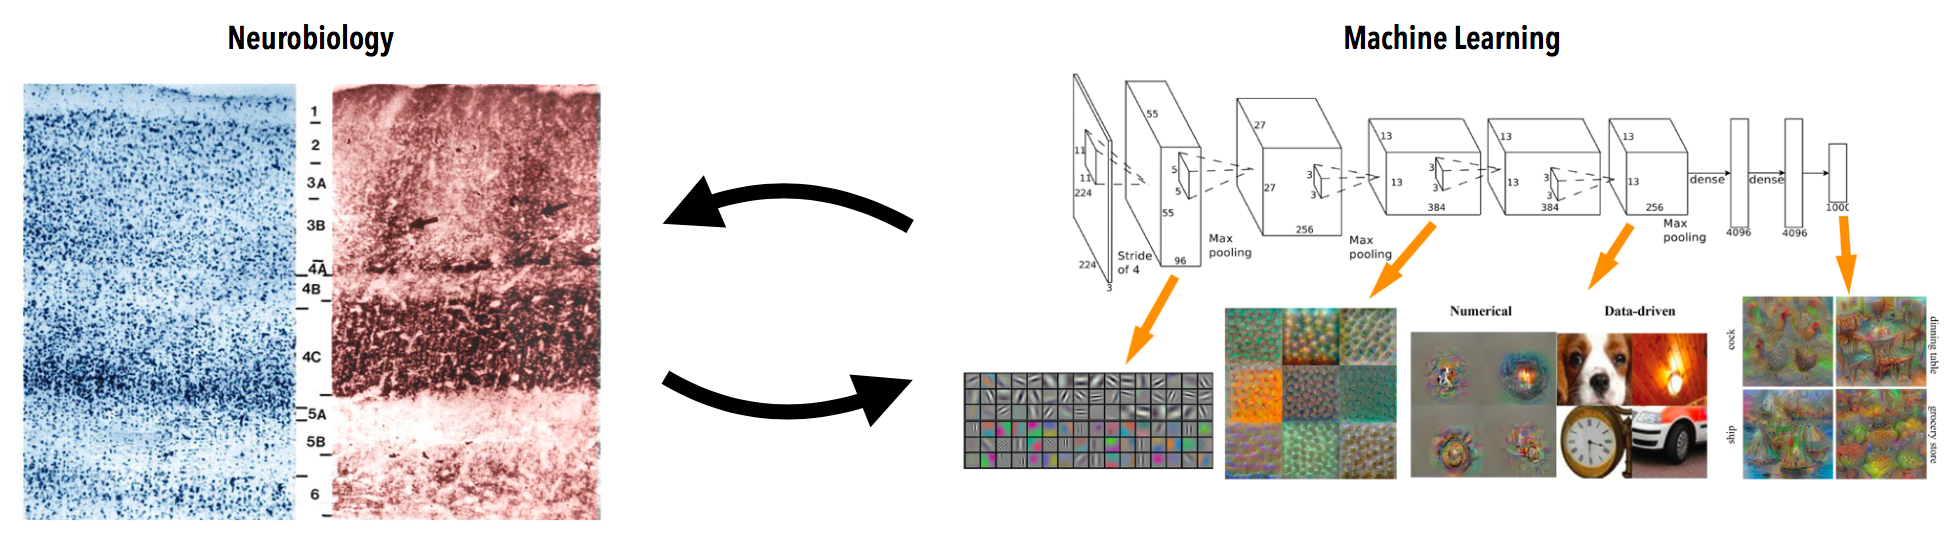
\includegraphics[width=\linewidth]{biology_vs_cnn.png}
%  \caption{The Biological Vision (schematic)}
%	\label{fig:vision}
%\end{figure}

Biological vision is an extremely powerful system which allows humans the ability, and seemingly without effort, to recognize an enormous amount of distinct objects in the world. 
Object detection is extremely difficult and therefore is especially impressive as light intensities can change by levels of magnitude and contrast between foreground and background is so often low. 
In addition, the visual scene changes every time the human body or human eyes move. 
This visual system exhibits a very noisy structure but because it is organized by layers it has inspired the mathematical theory of multilayer neural networks. 
What is remarkable is that even though current machine learning models do not resemble the complexity of its biological pendant, they inherently generalize extremely well. 
Neural networks trained on one specific task can be used to perform detection or segmentation of, seemingly, unrelated objects with relatively minor retraining. 
The reported classification performance is superior to that of humans and the question in regards to their functionality opens an interesting research topic.

In 1962 Hubel and Wiesel were the first to begin studying the visual cortex from the standpoint of a neuroscientist. Their experimental findings on cats and macaque monkeys suggested a hierarchy of cells with increasing complexity which was then later transferred to the hierarchical model of different layers. Twenty years later, this insight was translated to the Neocognitron quantitative model, by Fukushima and Miyake, which ultimately led to the important work of Hinton, Bengio, and LeCun in the 1980s. Their work on stochastic gradient descent approximation, and the availability of faster computer hardware then led to today’s breakthrough of deep learning networks. In the last decade, this field has exhibited rapid growth, constant evolution, and new applications in various domains.

We think that the biological inspiration of modern convolutional neural networks yields the evaluation of principles of human perception with computers.


